\section{ネットワークの変更}
春山らの先行研究では,\figref{fig:haruyama_net}に示すネットワークを使用していた.
一方でfelipeらの先行研究によると,コマンドによってモデルを分岐する形式のネットワークがより経路追従の成功率が向上すると報告している.
そのため,今回の研究ではfelipeらによって提案されたネットワークを参考に\figref{fig:branched}に示す,新たなネットワークを構築した.

\begin{figure}[htbp]
  \centering
  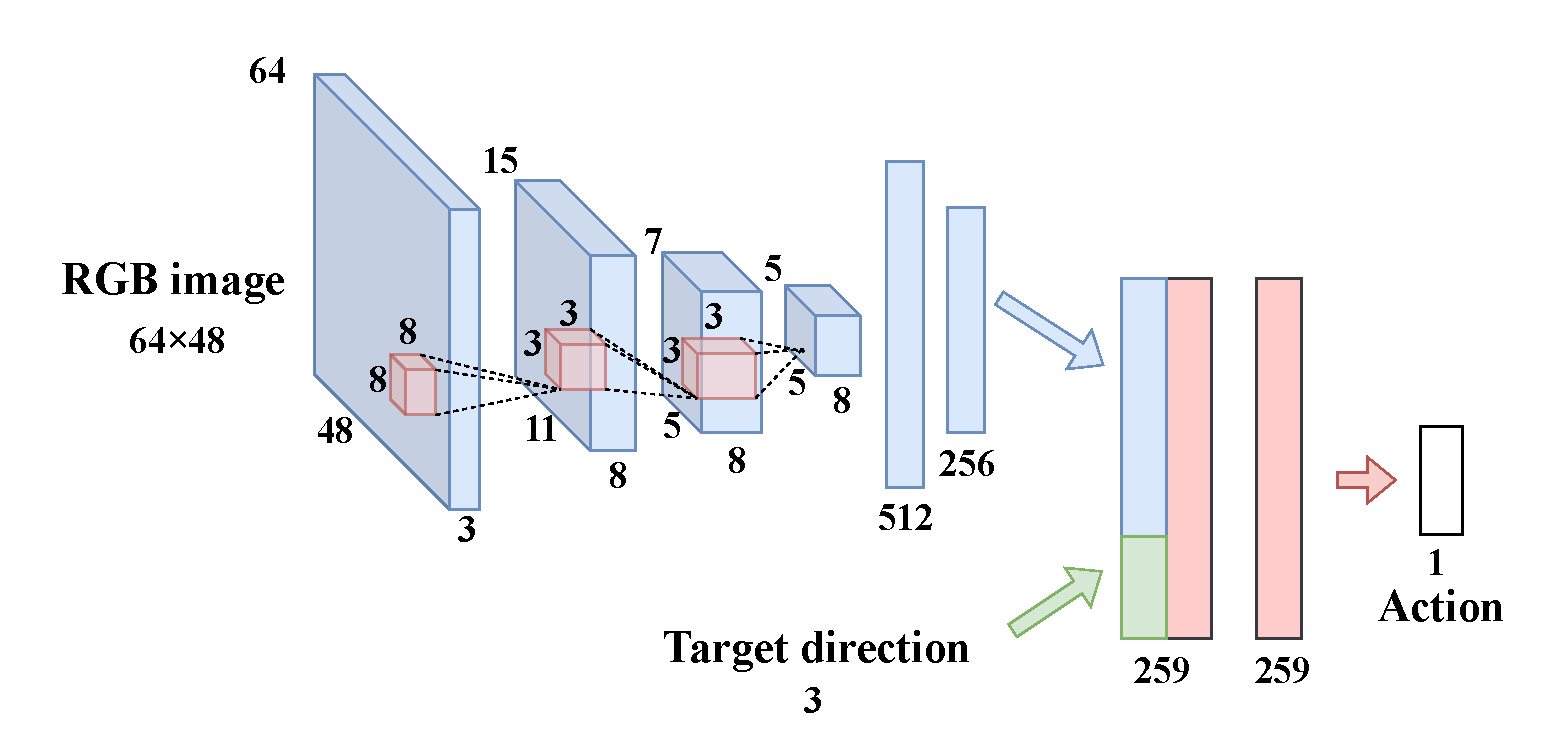
\includegraphics[width=100mm]{images/pdf/haruyama/net.pdf}
  \caption{Structure of the network(Quoted from \cite{fujiwara2023})}
  \label{fig:haruyama_net}
\end{figure}

\begin{figure}[htbp]
  \centering
   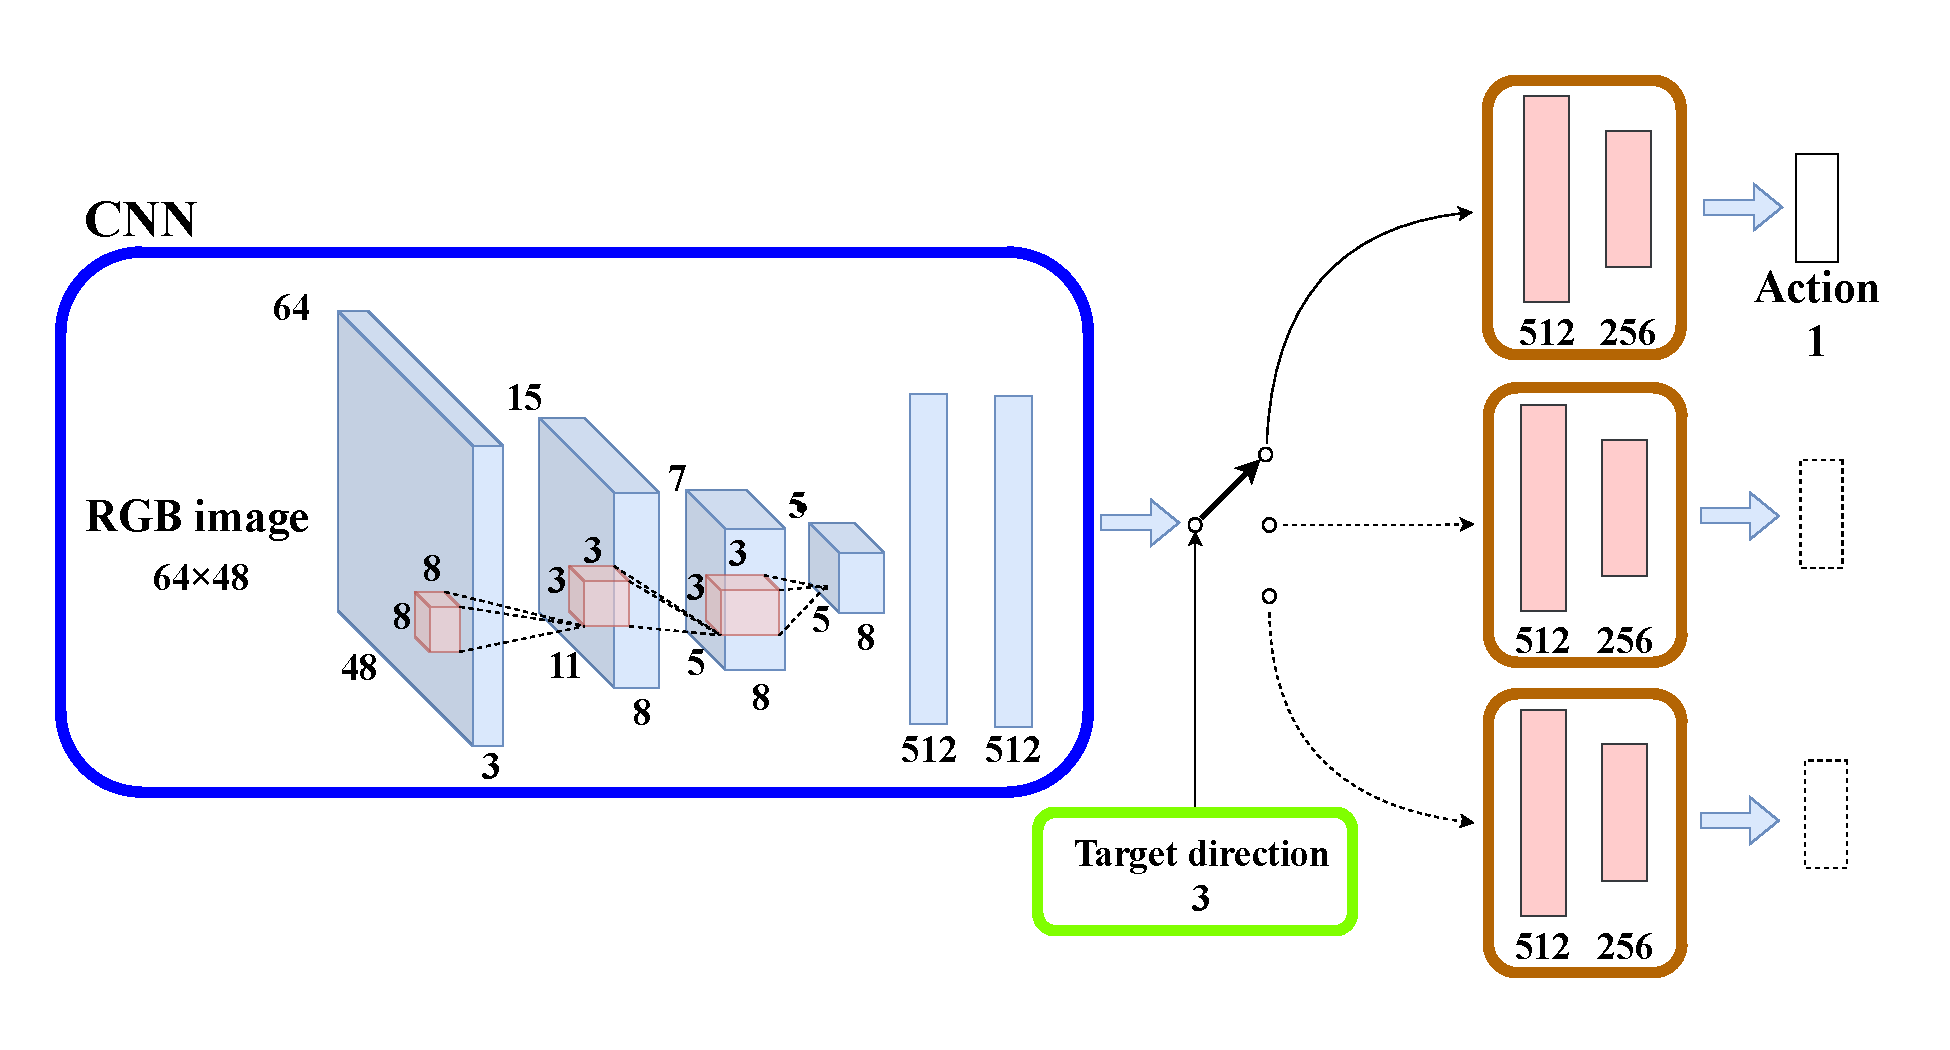
\includegraphics[width=100mm]{images/pdf/ishiguro/branched.pdf}
   \caption{Branched network}
   \label{fig:branched}
\end{figure}